\documentclass[a4paper,10pt]{report}
\usepackage[francais]{babel}
\usepackage[utf8]{inputenc}
\usepackage{graphicx}
\usepackage{array}
\usepackage{caption}
\usepackage{subcaption}
\usepackage{float}
\newcommand{\HRule}{\rule{\linewidth}{0.5mm}}
\setcounter{secnumdepth}{3}
\setcounter{tocdepth}{3}

\date{2014-2015}

\begin{document}

\begin{titlepage}
 \begin{center}

 \begin{minipage}{0.4\textwidth}
    \begin{flushleft} \large
        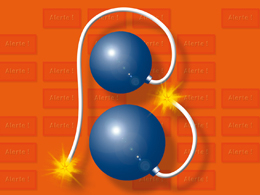
\includegraphics[width=3cm]{image/bonsai.jpg}
    \end{flushleft}
  \end{minipage}
  \begin{minipage}{0.4\textwidth}
    \begin{flushright} \large
      
\includegraphics[width=3cm]{image/lille1.png}
    \end{flushright}
  \end{minipage} 
  ~\\[3cm]

  \textsc{\LARGE PJI\\ Master 1 informatique}\\[1.5cm]

  \textsc{\Large Université Lille 1}\\[0.5cm]

  % Title
  \HRule \\[0.5 cm]
  { \huge \bfseries Prédiction de l'activité des peptides\\[0.8cm] \large \emph{CRISTAL - Equipe BONSAI} \\[0.4cm] }
  \HRule \\[1.5 cm]

  % Author and supervisor
  \begin{minipage}{0.4\textwidth}
    \begin{flushleft} \large
      \emph{Auteur:}\\
	Emilie \textsc{Allart}
    \end{flushleft}
  \end{minipage}
  \begin{minipage}{0.4\textwidth}
    \begin{flushright} \large
      \emph{Tuteurs:} \\
      Maude \textsc{Pupin} \\
      Laurent \textsc{Noé}
    \end{flushright}
  \end{minipage} 

  \\[3cm]
  {\large \emph{9 mars 2015} }
  \vfill
 \end{center}
\end{titlepage}


  \newpage
  \tableofcontents 
  \newpage

  \section*{Introduction}

      \paragraph
      \\
      ~~\\Au cours de la première année de master informatique, nous avons la possibilité de choisir dans le cadre du module PJI un projet à effectuer dans un laboratoire de recherche.
      J'ai donc effectué le mien au sein de l'équipe Bonsai, une équipe orientée bioinformatique faisant partie de CRISTAL. 
      
      ~~\\ Bonsai est un groupe de recherche en bioinformatique affilié avec INRIA Lille - Nord Europe et le Centre de Recherche en Informatique, Signal et Automate de Lille (CRIStAL, Université Lille 1, CNRS).
      Leur objectif principal est de définir des modèles et des algorithmes efficaces pour l'analyse de séquence à grande échelle dans le dommaine de la biologie moléculaire. Cela comprend par exemple la génomique comparative et la métagénomique .
      
      Une branche en particulier est orientée vers les peptides non ribosomiques (ou NRPs) dirigée par Maude Pupin.  
     
      C'est pourquoi, encadrée par Maude Pupin et Laurent Noé, j'ai travaillé sur le thème de : \textit{Rechercher les meilleurs critères pour la prediction de l'activité d'un peptide}.
      Ceci rejoint une étude menée auparavant par l'équipe, intitulée \textit{A new fingerprint to predict nonribosomal peptides acitvity}, qui étudie la décomposition d'un NRP en monomères (sous-ensemble) pour prédire son activité.
     
      Nous allons donc étudier les peptides de la base Norine et d'essayer de trouver de nouveaux critères pour améliorer la prédiction de l'activité d'un peptide. De plus, une automatisation du programme permettra aux personnes le souhaitant d'utiliser leur base d'apprentissage.
      ~~\\Le but est de pouvoir par la suite prédire l'activité d'un peptide inconnu, avec pour information sa composition en monomères et sa structure. Et d'élever les résulats par rapport à la précédente recherche.
     
     
      ~~\\Dans ce rapport, nous allons expliquer ce qu'est un NRP et présenter Norine, puis annoncer le plan du projet. Dans une deuxième partie, nous détaillerons étape par étape le travail effectué. Et enfin nous présenterons les résultats obtenus avec un comparatif de l'étude précédente, et les réponses que l'on peut en tirer.
     
      \addcontentsline{toc}{section}{Introduction}
      \newpage


  \chapter{Contexte}

    
    \section{NRP}
      \begin{figure}[h]
	\caption{Décomposition monomérique de ...}
	\includegraphics[scale = 0.5]{}
      \end{figure}
      \paragraph{}
	~\\ 
	Les bactéries et les champignons comportent des peptides synthétisés par une voie indépendante du ribosome. 
	Ils ne suivent pas la voie classique allant de la transcription de l'ADN, à la traduction de l'ARN en peptide sur le ribosome.
	Ils utilisent une voie alternative utilisant des NRPSs (ou non-ribosomal peptide synthetase) qui sont des complexes multi-enzimatiques organisés en module.
	Les NRPs sont des composés chimiques synthétisés par de grandes enzymes qui regroupent des acides aminés mais aussi des dérivés et autres (des lipides ou des glucides par exemple). Ils sont associés par des liaisons peptidiques et non peptidiques. 
	
	\\Les NRPs servent déjà à fournir des médicaments mais leur capacité à fournir de nouveaux médicaments et produits pharmacologiques n'est pas encore assez exploitée. Il faut continuer à en découvrir de nouveaux et en apprendre d'avantage sur leurs activités.

      \subsection{Monomère}
	
	~~\\Pour mieux comprendre les NRPs, une décomposition en monomère a été mise en place. 
	Comme dit auparavant, un NRP est un assemblage d'acides aminés mais aussi de lipides et glucides, que nous  appelons monomères (les unités de base) . 
	Un NRP a la spécificité d'être de petite taille (2 à 50 monomères) et d'être fort diversifié car il existe plus de 500 monomères comptant les 21 acides aminés et tous les dérivés.
	Ainsi, on peut décrire un NRP par l'ensemble des monomères qui le composent et en tirer des informations. 
	
	\\Voici la décomposition monomérique du alamethicin F50 : Ac-Aib, Pro, Aib, Ala, Aib, Ala, Gln, Aib, Val, Aib, Gly, Leu, Aib, Pro, Val, Aib, Aib, Gln, Gln, Pheol
	
      \subsection{Structure}
	
	~~\\Ainsi il est plus aisé de représenter un NRP sous la forme d'un graphe avec pour noeuds les monomères qui le constituent, et pour liens les liaisons qui les relient.
	Le NRP ne contient pas seulement des liaisons peptidiques, mais également des liaisons non-peptidiques. Cela engendre donc l'apparition possible de structures cycliques (partielles ou non) et de ramifications sur la structure primaire de la molécule. 
	
	Grâce à la structure du NRP (graphe), on peut décrire les liens entre les monomères et analyser l'effet qu'ils ont sur l'activité du peptide.
	C'est pourquoi, dans le projet, l'arité de chaque monomère, c'est-à-dire le nombre de liaisons que possède un monomère, est étudier.
	
	On peut décrire cette structure par une description linéaire qui liste les monomères dans un ordre, permettant d'identifier un monomère par sa position, et à la suite, à l'aide de symboles '@', se trouve les liens qui existent entre eux
	
	\\TODO : exemple de description linéaire avec explication
	
	\subsection{Activité}
	
	En effet, les NRPs sont une mine d'or pour les biologistes, ils ont un large domaine d'activité au niveau biologique et pharmacologique. 
	Ils peuvent, par exemple, avoir comme activité:
	\begin{itemize}
	 \item antibiotique : lutte contre les bactéries \textit{ex : ACV (précurseur de la penicilline)}  
	 \item anticancéreux : lutte contre le cancer \textit{ex : actinomycin D}
	 \item toxine :  tue les cellules \textit{ex :callipeltin D}
	 \item sidérophore : agit comme un aimant avec les molécules de fer \textit{ex : amphibactin I}
	 \item inhibiteur de la protéase : lutte contre les virus \textit{ex : cyanostatin B}
	\end{itemize}
	Un NRP peut posséder plusieurs activités à la fois, mais nous ne considerons que ceux qui ne possèdent qu'une seule activité.
       
      \subsection{Clusters}
      
	Bien souvent les monomères partagent des propriétés physico-chimiques, soit parce qu'ils ont une structure similaire, soit parce qu'ils dérivent tous d'un même composant auquel s'est ajouté un groupement ( groupement acetyl, methyl, etc...), ou qui a changé de conformité. Cela nous permet de les ranger dans des clusters (ou des familles).
	
	Ainsi, nous examinons ces clusters et regardons s'ils peuvent nous aider à améliorer la prediction de l'activité d'un peptide.
	
	Voici l'exemple du rangement en cluster que nous avons utilisé :
	
	\begin{description}
	 \item[Chromophores non siderophore] \hfill \\ChrD;ChrA;ChrAct
	 \item[Siderophores] \hfill \\ChrI;ChrP;OH-Asp;D-OH-Asp;OH-His;Ac-OH-Orn;D-Fo-OH-Orn;D-OH-Orn;D-Ac-OH-Orn;D-OH-cOrn;OH-Orn;NAc-Fo-OH-Orn;Fo-OH-Orn;OH-cOrn
	 \item[Peptaibols (antibiotiques)]\hfill \\ NAc-Dpr;Ac-Ser;Ac-Ival;Ac-Val;Ac-Trp;Ac-Phe;Ac-Aib;NAc-Leu;Ivalol;Leuol;Valol;Ileol;Pheol;Trpol;Serol;OAc-Leuol;Aib;Ival;4OH-Pro;Et-Nva
	 \item[Hpg et derives (antibiotiques)] \hfill \\Hpg;D-OH-dHpg;Cl2-Hpg;NMe-Hpg;Cl-Hpg;OH-dHpg;D-Hpg
	 \item[Sucres (antibiotiques)] \hfill \\2OMe-Rha;Ara;Aco;D-Gal;D-Ara;Ere;Glc;Oli;D-Glc;bD-Gal;U4oxo-Van;Rha;D-Man;4oxo-Van;Act;Lyx;Ria;Van
	\end{description}

	
	  
      \section{Norine}
	
	\paragraph{}
	  
	  \\Norine (NOnRibosomal peptides with INE) est une plateforme contenant la première base de données entièrement dédiée aux peptides non ribosomiques, elle répertorie 1174 NRPs et pas moins de 528 monomères. Elle fournit aussi les outils permettant le traitement de ces NRPs. 
	  Le site est organisé en plusieurs parties, une partie 'peptide' présente pour un peptide donné son nom, ses synonymes, les activités biologiques, sa formule moléculaire, sa formule monomérique , etc...; une autre partie 'structure' où l'on retrouve les peptides classés par type (cyclique, linéaire, double cyclique, ...), qui donne la structure monomérique des peptides.
	  On peut également trouver la description des monomères. 
	   
	\begin{figure}[h]
	  \caption{Capture de la descritpion d'un peptide sur Norine}
	  \includegraphics[scale = 0.5]{}
	\end{figure}
	\\ TODO Description de la capture ... 
    
	
      \section{Problématique}
	
	\paragraph{}
	  Les NRPS , bien que fort intéressant, sont difficile à produire et à analyser. On ne peut donc pas utiliser les méthodes habituelle d'analyse de forme 3D ou de leur reaction physico-chimique.
	  C'est pourquoi le but de l'étude précédente est de donner des modèles de prediction informatique permettant de prédire l'activité d'un peptide.
	  Ces modèles se basaient uniquement sur l'empreinte monomérique du peptide, c'est-à-dire un comptage de chaque monomère pour voir lesquels sont présent et en déterminer d'après l'apprentissage quel 'schéma' il suit.

	  Pour notre part , nous ajouterons d'autres critères, à savoir l'occurence des clusters de monomères et le comptage des liens.
	  Puis, par le biais de méthodes d'apprentissage et de validation croisée, nous chercherons à voir lequel ou lesquels de ces critères prédisent au mieux l'activité du peptide concerné.
	  
	  Dans l'idéal, nous aurons de meilleurs modèles pour prédire l'activité d'un peptide. Nous comparerons les différents résulats entre eux et avec ceux de l'autre étude, pour trouver les meilleurs critères.
	
	
      \section{Plan}
	
	\begin{figure}[h]
	  \caption{Schéma des étapes à suivre}
	  \includegraphics[scale = 0.5]{}
	\end{figure}
	  \\TODO  Récupération et filtrage des données -> Préparation des données selon les critères -> Apprentissage -> Etude des résultats 
   
  \chapter{Mise en oeuvre}

  
    \section{Récupération depuis Norine}
    
	Norine met à diposition une passerelle REST, nous permettant de récupérer plus facilement les données.
	De cette façon, par l'intermédiaire de fichier JSON, nous avons récupéré les informations sur chaque peptide nous intéressant, ainsi que la liste de tous les monomères de la base.
	
	    
	~\\ Sur chaque peptide, si toutes les données sont fournies, nous conservons son identifiant (NOR suivi de 5 chiffres), sa composition monomérique, son activité et sa structure linéaire. 
	    
	Pour rester cohérent avec l'étude précédente, nous avons enlevé une activité redondante 'surfactant' et nous ne conservons que les peptides ayant une seule activité.
	Nous avons également créé un filtre qui ne garde que les peptides dont l'activité est assez représentative, elle doit dépasser un certain seuil que nous fixons.
      
	Une fois les données récupérées, nous les traitons selon les critères que nous souhaitons tester.   
   
    \section{Création des empreintes}
	
	Une fois les données récupérées de Norine et filtrées, nous faisons les empreintes selon ce que l'on veut tester.
	
	\paragraph{Empreinte en monomère}
	    ~\\
	    Au préalable nous avons prélèvé l'ensemble des monomères de Norine.
	    
	    A chaque peptide, nous comptons le nombre d'occurences de chaque monomère dans sa composition et en faisons ainsi une empreinte.
	    
	    \begin{figure}[h]
	      \caption{Exemple d'empreinte en monomère}
	      \includegraphics[scale = 0.5]{}
	    \end{figure}
	    
	\paragraph{Empreinte en cluster}
	~\\
	  De même que pour les monomères, nous devons au préalable charger un fichier répertoriant les clusters de monomères avec leur nom et les monomères qui les composent.
	  
	  C'est le même principe qu'auparavant, nous faisons l'empreinte mais cette fois nous notons le nombre d'occurences d'un cluster en comptant combien de fois les éléments de celui-ci apparaissent dans ce peptide.
	 
	  
	\paragraph{Empreinte en lien}
	    ~\\
	    Comme dit précédemment, les NRPs sont représentés par des graphes de monomères. On peut donc intégrer la notion d'arité, qui représente le nombre de lien que possède un sommet, donc pour notre problème, cela représente le nombre de monomères auquel est lié un monomère. 
	    Pour chaque arité, allant de 1 à 5, nous comptons le nombre de sommets ayant cette arité. Cela nous permet de faire l'empreinte. 

	\paragraph{}
	  ~\\
	  Selon les critères que nous voulons tester, nous ajoutons à la liste pour chaque peptide leur(s) empreinte(s).
	  Nous pouvons tester les critères seules ou associés, par exemple les liens et les monomères ensemble ou alors les clusters seuls.
	  
     \section{Lancement des méthodes d'apprentissage}
	  
	  ~\\
	  Pour traiter les données, nous utilisons 3 méthodes d'apprentissage : le naïveBayes, le SMO et le LibLinear. 
	  
	  Pour cela, nous avons utilisé des librairies python et une extension pour LibLinear qui n'est pas implémentée de base.
	  
	  Le programme prend en entrée le fichier contenant les données et donne en sortie les mesures de robustesse à analyser.
	  
	  
	  ~\\Le Naïve Bayes repose sur le théorème de Bayes, il possède une phase d'entrainement et une phase de test.
	  On fait de l'apprentissage probabiliste sur l'ensemble des peptides, ainsi lorsque l'on teste à quelle activité appartient un nouveau peptide, on prend celle qui a la plus grande probabilité.  
	    
	  Le SMO est une méthode d'apprentissage supervisé qui construit au fur et à mesure de la lecture des données une fonction objective via une descente de gradient.   
	  LibLinear reste dans la même idée.
	      
	  \paragraph{Validation croisée}
	    
	  Nous divisons les peptides en 10 groupes, nous faisons un apprentissage des empreintes sur 9 groupes et testons sur le dernier groupe si l'activité que l'on trouve correspond bien. Nous faisons cela pour chacun des groupes et obtenons ainsi des mesures de qualités.
	    
     \section{Mesures de robustesse}
	  
	  ~\\
	  Nous obtenons ainsi un ensemble de mesures de robustesse qu'il faut comparer pour voir quel critère ou quel combinaison de critère est la plus efficace pour obtenir des informations sur un peptide.
	  Pour notre étude, nous utilisons la précision, la sensibilité, la F-measure et le ROC.
	     
	     \paragraph{Precision}\\
	      
	     ~\\ 
	     La précision se calcule en divisant le nombre d'éléments bien classés par le nombre d'éléments en tout.
	     Dans notre cas, elle se calcule en divisant le nombre de peptides bien classés par le nombre de peptides traités.
	     Elle est la probabilité que les données soient bien triées, une mesure de la qualité de la classification. 
	     Donc un taux élevé est attendu dans la recherche.
	     \[ 
	      précision = \frac{ elements correctement attribues à la classe i }{ nombre d'elements attribues a la classe i }
	     \]

	     
	     \paragraph{Sensibilité}
	     
	     ~\\
	     La sensibilité se calcule en divisant le nombre d'éléments bien classés pour une classe donnée sur le nombre de données de cette classe. 
	     Cela représente le nombre de peptides bien annotés pour une activité par rapport au nombre de peptides rangés dans cette activité.
	     Elle prend une valeur entre 0 et 1, plus elle tend vers 1 plus la classification est bonne.
	     \[
	      sensibilite = \frac{ elements correctement attribues à la classe i }{ nombre d'elements appartenant a la classe i }
	     \]

	     \paragraph{F-measure}\\
	     
	     ~\\La F-measure allie la précision et la sensibilité, ainsi si elle approche 1 c'est un bon résulat.
	     \[
	      f-measure = \frac{ 2 \times precision \times sensibilite }{ precision + sensibilite }
	     \]
	     \paragraph{AUC ou ROC}\\
		
	     ~\\La courbe ROC est la courbe représentant les faux-positifs (valeur rangée dans une classe alors qu'elle n'en fait pas partie) en fonction des vrai positifs (valeur bien rangée).
	     
	 
   \chapter{Résultats}

	  
      \section{Résultats obtenus}
	 
	  
	  Faire ces tableaux pour les meilleurs résultats
	  Puis comparatif avec graphes ? 
	  \paragraph{}
	   \begin{flushleft}
	    \leftskip -3cm
	    \begin{tabular}{|l|l|l|l|l|l|l|l|l|l||l|l|l|}\hline
	      \multirow{2}{|l|}{Activite} & \multicolumn{4}{|l|}{Naive Bayes} & \multicolumn{4}{|l|}{LibLinear} & \multicolumn{4}{|l|}{SMO} \\\cline{2-13}
	       & Prec & Rec & F & AUC & Prec & Rec & F & AUC & Prec & Rec & F & AUC & \\\hline
	      Antibiotique & . & . & . & . & . & . & . & . & . & . & . & . & \\\hline
	      Toxine & . & . & . & . & . & . & . & . & . & . & . & . & \\\hline
	      Siderophore & . & . & . & . & . & . & . & . & . & . & . & . & \\\hline
	      Anticancereux & . & . & . & . & . & . & . & . & . & . & . & . & \\\hline
	      Inhibiteur protease & . & . & . & . & . & . & . & . & . & . & . & . & \\\hline
	    \end{tabular}
	  \end{flushleft}
	  
	  
	  Conclusion : quelles sont les meilleures combinaisons ... 
      
      \section{Comparaison avec les résultats précédents}
      
	  TODO tableau et/ou graphe comparatif
	  
	  Conclusion : Avons-nous avancé depuis l'étude précédente? Quelles sont les meilleurs critère ou combinaison de critères pour déterminer l'activité d'un peptide ? 
    
  \section*{Conclusion}
     
    \phantomsection
    \addcontentsline{toc}{section}{Conclusion}
    \newpage

    Pour rappel, notre problématique était de chercher des meilleurs critères pour déterminer l'activité d'un peptide. 
    A savoir que le programme est conçu pour que toutes personnes le souhaitant puisse faire l'apprentissage sur ses données.
    
    TODO après résultats
   
    En comparant, les résulats de l'étude effectuée sur les NRPs de Norine quelques années auparavant et les résultats que nous avons obtenus en combinant différentes connaissances sur ces NRPs, nous avons trouver des combinaisons de critères nous permettant d'apprendre avec plus de certitudes l'activité d'un NRP. 
    Pour connaitre l'activité d'un NRP avec une certitude de ... minimum, il faut combiner .... 
    
    Nous avons donc pu aller au bout de ce projet, en trouvant une combinaison meilleur, ne reste plus qu'à analyser de nouveau NRP pour, qui sait, trouver un nouvel antibiotique ...  
    \newpage
    
    \section*{Glossaire}
    
    \phantomsection
    \addcontentsline{toc}{section}{Glossaire}
    \newpage
    
   
    \newpage
   
    \section*{Références}
     \end{itemize}

    \phantomsection
    \addcontentsline{toc}{section}{Annexe}
    \newpage

  \end{document}          
